\documentclass[a4paper, 14pt]{article}
\usepackage[utf8x]{inputenc}
\usepackage[russian]{babel}
\usepackage{graphicx}
\usepackage{listings}
\usepackage{color}
\usepackage{amsmath}
\usepackage{pgfplots}
\usepackage{url}
\usepackage{flowchart}
\usepackage{tikz}
\usepackage{mathtext} 
\DeclareGraphicsExtensions{.pdf,.png,.jpg,.svg}
\usetikzlibrary{shapes, arrows}

\usepackage[utf8]{inputenx}

\usepackage{geometry} 
\geometry{left=2cm} 
\geometry{right=1cm} 
\geometry{top=2cm} 
\geometry{bottom=2cm}

\usepackage{lipsum}
\setlength{\parindent}{8ex}
\usepackage{indentfirst}

\usepackage{titlesec}
\titleformat*{\section}{\LARGE\bfseries}
\titleformat*{\subsection}{\Large\bfseries}
\titleformat*{\subsubsection}{\Large\bfseries}
\titleformat*{\paragraph}{\Large\bfseries}
\titleformat*{\subparagraph}{\large\bfseries}
 
\begin{document}
	\thispagestyle{empty}
 	\begin{center}
 		\hfill \break
 		\textit{
 			\normalsize {\bf  Министерство науки и высшего образования Российской Федерации}\\
 			\normalsize {\bf Федеральное государственное бюджетное образовательное учреждение }\\
 			\normalsize {\bf  высшего  образования}
 			\normalsize  {\bf  «Московский государственный технический университет}\\ 
 			\normalsize  {\bf имени Н. Э. Баумана}\\
 			\normalsize  {\bf (национальный исследовательский университет)»}\\
 			\normalsize  {\bf (МГТУ им. Н.Э. Баумана)}\\
 		}
 		\noindent\rule{\textwidth}{2pt}
 		\hfill \break
 		\hfill\break
 		\hfill\break
 		\hfill\break
 		\hfill\break
 		\hfill\break
 		\hfill\break
 		\hfill \break
 		\hfill \break
 		\textit{
 			\normalsize {\bf РАСЧЕТНО-ПОЯСНИТЕЛЬНАЯ ЗАПИСКА}\\
 			\normalsize {\bf к курсовому проекту на тему:}\\
 			\normalsize {\bf  Поиск фильмов по параметрам и просмотр информации о них} \\
 		}
 		\hfill \break
 		\hfill \break
 		\hfill \break
 		\hfill \break
 		\hfill \break
 		\hfill \break
 		\hfill \break
 		\hfill \break
 		\hfill \break
 		\hfill \break
 		\hfill \break
 		
 		\hfill \break
 		\normalsize {
 			\noindent
 			\makebox[0pt][l]{Студент}%
 			\makebox[\textwidth][c]{}%
 			\makebox[0pt][r]{{$\underset{\text{(Подпись, дата)}}{\underline{\hspace{4cm}}}$ \space 
 					Полякова К. А.}}
 		}\\
 		\hfill \break
 		\hfill \break
 		\normalsize {
 			\noindent
 			\makebox[0pt][l]{Руководитель курсового проекта}%
 			\makebox[\textwidth][c]{}%
 			\makebox[0pt][r]{{$\underset{\text{(Подпись, дата)}}{\underline{\hspace{5cm}}}$ \space 
 					Филиппов М. В.}}
 		}
 		\hfill \break
 		\hfill \break
 		\hfill \break
 		\hfill \break\hfill \break
 		\hfill \break
 	\end{center}
 	\hfill \break
 	\hfill \break
 	\hfill \break
 	\hfill \break
 	\begin{center} Москва 2020\end{center}
	\newpage
	
	\tableofcontents
	
	\newpage
	\section*{Введение}
	\addcontentsline{toc}{section}{Введение}
	Еще пару десятков лет назад, чтобы посмотреть какой-либо фильм люди посещали кинотеатры или смотреть телевизор. Но тогда выбор был очень ограниченный - приходилось смотреть только то, что шло в кинотеатрах или показывали по телевизору.
	
	Современный же человек не имеет таких ограничений. С появлением Интернета огромное количество различных фильмов, сериалов, мультфильмов доступны каждому прямо из дома. Необходимо заметить, что и количество кинофильмов увеличилось в несколько раз. Как же не запутаться в таком многообразии и выбрать именно то, что нравится? Как раз для этого необходимы приложения для поиска по различным параметрам и для просмотра необходимой информации, чтобы найти определенный фильм.
	
	\hfill \break
	
	Целью данной курсовой работы является создание клиент–серверного приложения <<ХочуПосмотреть!>>, которое предоставляет возможность просмотра информации о различных фильмах. Также пользователь может добавить любые фильмы в Избранное для того, чтобы посмотреть их позже или пересмотреть. В приложении можно осуществить поиск по нескольким параметрам: по названию, по году премьеры, по стране или по жанру.
	
	Актуальность разработки состоит в том, что с помощью такого приложения можно с легкостью найти информацию о фильме или добавить фильм в Избранное, чтобы не забыть его посмотреть.
	
	Для выполнения цели необходимо выполнить следующие задачи:
	\begin{itemize}
		\item формализовать задачу в виде определения необходимого функционала;
		\item провести анализ существующих средств управления базами данных (СУБД);
		\item спроектировать базу данных, необходимую для хранения и структурирования данных;
		\item реализовать спроектированную базу данных с использованием выбранной СУБД;
		\item реализовать приложение для взаимодействия с реализованной базой данных.
	\end{itemize}
	\newpage
	
	\section{Аналитический раздел}
	В данном разделе будут рассмотрены общие сведения о базах данных и средствах управления базами данных, типы баз данных и используемые framework'и. 
	
	\subsection{Формализация задачи}
	
	В соответствии с техническим заданием на курсовой проект пользователям необходима система авторизации и регистрации для предоставления индивидуальной информации.
	
	Также должна быть предусмотрена возможность поиска и просмотра информации о фильмах, а также добавление в Избранное и удаление фильмов из Избранного.
	
	\subsection{Общие сведения о базах данных и средствах управления базами данных}%
	
	База данных представляет собой совокупность определенным образом организованных данных, которые хранятся в памяти вычислительной системы и отображают состояние объектов и их взаимосвязи в рассматриваемой предметной области.\\
	Под системой управления базами данных (СУБД) понимается совокупность программных и языковых средств, предназначенных для создания и обработки БД. 
	
	\subsection{Типы БД}
	
	Модель данных определяет логическую структуру БД и то, каким образом данные будут храниться, организовываться и обрабатываться. 
	
	Существует 3 типа моделей организации данных:
	\begin{itemize}
		\item иерархическая модель БД;
		\item сетевая модель БД;
		\item реляционная модель БД.
	\end{itemize}
	
	\subsubsection{Иерархическая модель баз данных}
	
	Иерархическая модель БД представляет собой древовидную (иерархическую) структуру, состоящую из объектов (данных) различных уровней. Каждый объект может включать в себя несколько объектов более низкого уровня. Такие объекты находятся в отношении предка (объект более близкий к корню) к потомку (объект более низкого уровня), при этом возможна ситуация, когда объект-предок имеет несколько потомков, тогда как у объекта-потомка обязателен только один предок.
	
	Иерархической базой данных является файловая система, состоящая из корневого каталога, в котором имеется иерархия подкаталогов и файлов.
	
	Связи записей реализуются в виде физических указателей с одной записи на другую. Основной недостаток иерархической структуры – невозможность реализовать отношения "многие-ко-многим", а также ситуации, в которых запись имеет несколько предков. \cite{0}
	
	\begin{figure}[h]
		\center{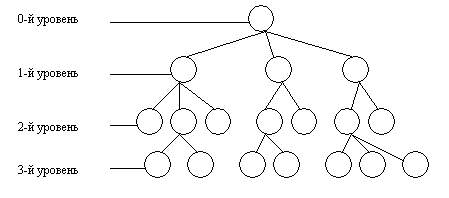
\includegraphics[scale=0.65]{img/1.jpg}}
		\caption{Иерархическая модель баз данных}
		\label{fig:image}
	\end{figure}
	
	\subsubsection{Сетевая модель баз данных}
	
	Сетевая модель данных является расширением иерархического подхода. 
	Разница между иерархической моделью данных и сетевой заключается в том, что в иерархических структурах запись-потомок должна иметь в точности одного предка, а в сетевой структуре у потомка может быть любое число предков. 
	Записи в такой модели связаны списками с указателями.
	
	Примером сетевой СУБД является IDMS (интегрированная система управления данными) от компании Computer Associates international Inc.
	
	Популярность сетевой модели совпала с популярностью иерархической модели. 
	Некоторые данные намного естественнее моделировать с несколькими предками для одного дочернего элемента. 
	Сетевая модель позволяла моделировать отношения «многие-ко-многим».
	
	И хотя эта модель широко применялась на практике, она так и не стала доминантной по двум основным причинам. 
	Во-первых, компания IBM решила не отказываться от иерархической модели в расширениях для своих продуктов, таких как IMS и DL/I. 
	Во-вторых, через некоторое время ее сменила реляционная модель, предлагавшая более высокоуровневый, декларативный интерфейс. \cite{0}
	
	\begin{figure}[h]
		\center{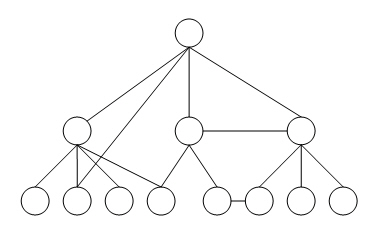
\includegraphics[scale=0.7]{img/2.jpg}}
		\caption{Сетевая модель БД}
		\label{fig:image}
	\end{figure}
	
	\subsubsection{Реляционная модель}
	
	В реляционной модели, в отличие от иерархической или сетевой, не существует физических отношений. Вся информация хранится в виде таблиц (отношений), состоящих из рядов и столбцов. А данные двух таблиц связаны общими столбцами, а не физическими ссылками или указателями. Объекты и их отношения представлены таблицами.
	
	В реляционных моделях нет необходимости просматривать все указатели, что облегчает выполнение запросов на выборку информации по сравнению с сетевыми и иерархическими БД. Это одна из основных причин, почему реляционная модель оказалась более удобна.
	
	\begin{figure}[h]
	\center{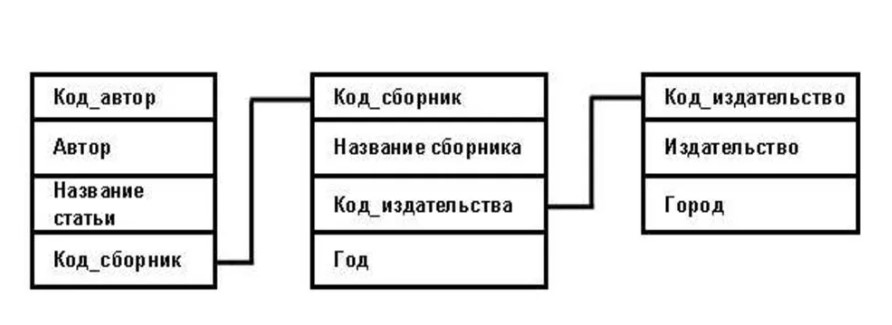
\includegraphics[scale=0.7]{img/3.jpg}}
	\caption{Пример реляционной БД}
	\label{fig:image}
	\end{figure}
	
	Распространенные реляционные СУБД: MySql, PostgreSql, Access, Oracle, DB2, MS-SQL Server, SQLite.
	Каждая реляционная таблица представляет собой двумерный массив и обладает следующими свойствами:
	
	\begin{itemize}
		\item каждый элемент таблицы — один элемент данных;
		\item все элементы в одном столбце имеют одинаковый тип;
		\item каждый столбец имеет уникальное имя;
		\item одинаковые строки (записи, кортежи) в таблице отсутствуют;
		\item порядок следования строк и столбцов может быть произвольным.
	\end{itemize}
	
	Каждое поле содержит одну характеристику объекта предметной области. В записи собраны сведения об одном экземпляре этого объекта.
	
	Некоторые поля могут быть определены как ключевые. Это значит, что для ускорения поиска конкретных значений будет использоваться индексация. Когда поля двух различных таблиц получают данные из одного набора, можно использовать оператор JOIN для выбора связанных записей двух таблиц, сопоставив значения полей. Такие действия можно расширить до объединения нескольких полей в нескольких таблицах. Поскольку отношения здесь определяются только временем поиска, реляционные базы данных классифицируются как динамические системы. 
	
	\subsubsection{Сравнение моделей}
	
	Иерархическая модель данных поддерживает отношения типа «один-к-одному» или «один-ко-многим». Она позволяет быстро получать данные, но не отличается гибкостью. Иногда роль элемента (родителя или потомка) неясна и не подходит для иерархической модели.
	
	Вторая, сетевая модель данных, имеет более гибкую структуру, чем иерархическая, и поддерживает отношение «многие ко многим». Но быстро становится слишком сложной и неудобной для управления.
	
	Третья модель – реляционная – более гибкая, чем иерархическая и проще для управления, чем сетевая. Реляционная модель сегодня используется чаще всего, так как имеет множество преимуществ, таких как:
	
	\begin{itemize}
		\item простота использования;
		\item гибкость;
		\item независимость данных;
		\item безопасность;
		\item простота практического применения;
		\item слияние данных;
		\item целостность данных.
	\end{itemize}
	
	В связи с этим далее будет рассматриваться реляционная модель. Теперь необходимо рассмотреть систему управления такой моделью.
	
	\subsection{СУБД}
	
	Самых популярные системы управления реляционными базами данных:
	\begin{itemize}
		\item MySQL;
		\item PostgreSQL; 
		\item SQLite.
	\end{itemize}
	
	В данном проекте будет рассмотрена СУБД SQLite.
	
	Это компактная встраиваемая СУБД. Слово «встраиваемый» (embedded) означает, что SQLite не использует парадигму клиент-сервер, то есть движок SQLite не является отдельно работающим процессом, с которым взаимодействует программа, а представляет собой библиотеку, компонующуюся с программой, и движок становится составной частью программы. Таким образом, в качестве протокола обмена используются вызовы функций (API) библиотеки SQLite. Такой подход уменьшает накладные расходы, время отклика и упрощает программу.
	
	Однако SqLite популярна скорее в случаях, когда не требуется выносить базу данных на отдельную машину и данные требуется хранить в рамках одной операционной системы. Будучи файловой БД, она предоставляет отличный набор инструментов для более простой (в сравнении с серверными БД) обработки любых видов данных. \cite{1}
	\newpage
	Преимущества:
	
	\begin{itemize}
		\item {\bf Файловая.} Вся БД хранится в одном файле, что облегчает перемещение.
		\item {\bf Стандартизированная.} SQLite использует SQL, некоторые функции не используются (RIGHT OUTER JOIN или FOR EACH STATEMENT);
		\item {\bf Отсутствие пользовательского.} Продвинутые БД предоставляют пользователям возможность управлять связями в таблицах в соответствии с привилегиями, но у SQLite такой функции нет.
		\item {\bf Невозможность дополнительной настройки.} SQLite нельзя сделать более производительной, путем изменения настроек.
	\end{itemize}
	
	\subsection{Framework}
	
	SQLite совместима со множеством фреймворков, которые содержат в себе требуемые методы обращения к БД.
	
	В качестве web-framework был выбран Django, который предоставляет все необходимые инструменты для создания подобного проекта, так как предоставляет возможность для написания как frontend, так и backend для полноценного запуска приложения.
	
	Django — свободный фреймворк для веб-приложений на языке Python, использующий шаблон проектирования MVC \cite{mvc}. Проект поддерживается организацией Django Software Foundation.
	
	Сайт на Django строится из одного или нескольких приложений, которые рекомендуется делать отчуждаемыми и подключаемыми. Это одно из существенных архитектурных отличий этого фреймворка от некоторых других. Также, в отличие от других фреймворков, обработчики URL в Django конфигурируются явно при помощи регулярных выражений.
	
	Для работы с базой данных Django использует собственный ORM, в котором модель данных описывается классами Python, и по ней генерируется схема базы данных. \cite{2}
	
	\subsection{Вывод}
	
	В результате проведенного анализа в качестве модели данных была выбрана реляционная модель, в качестве средства управления базами данных – SQLite.
	
	Таким образом, подобрав необходимый набор инструментов для реализации web-приложения, можно приступить к проектированию решения поставленной задачи.
	\newpage
	\section {Конструкторский раздел}
	
	В соответствии с техническим заданием и аналитическим разделом должно быть получено полноценное приложение для взаимодействия с базой данных.
	
	\subsection{Проектирование диаграмм web-приложения}
	
	На рисунке \ref{use-case} представлена Use Case диаграмма приложения. Можно заметить, что на диаграмме два актора: администратор и пользователь. Администратор взаимодействует с базой данных, добавляет и удаляет записи.
	
	\begin{figure}[h!]
		\center{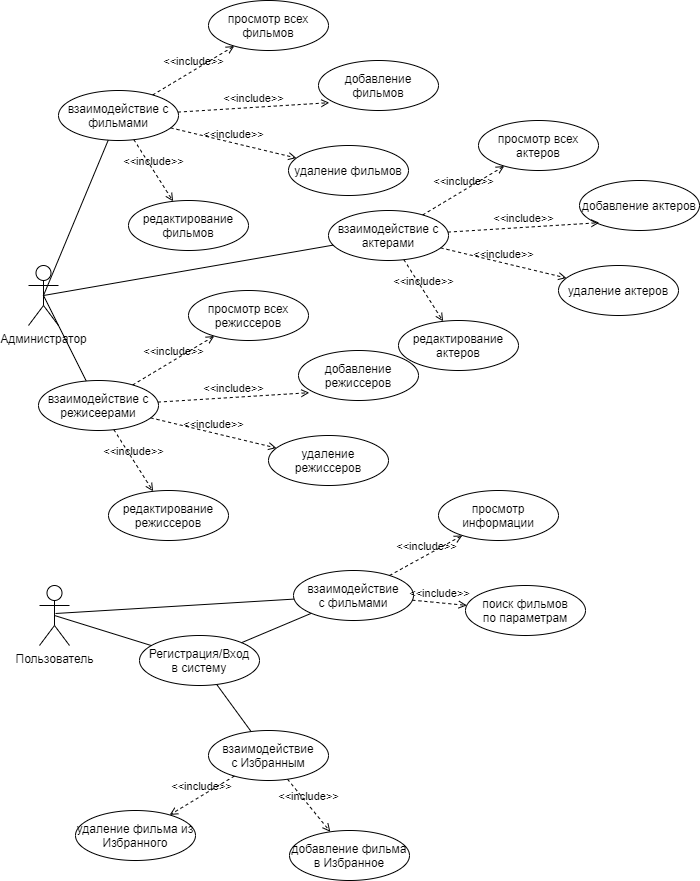
\includegraphics[scale=0.6]{img/use-case.png}}
		\caption{Use Case диаграмма}
		\label{use-case}
	\end{figure}

	\newpage
	На рисунке \ref{er-model} продемонстрирована ER модель приложения. Можно рассмотреть, какие сущности выделены, какая связь между данными ними и какие атрибуты присутствуют у каждой сущности.

	\begin{figure}[h!]
		\center{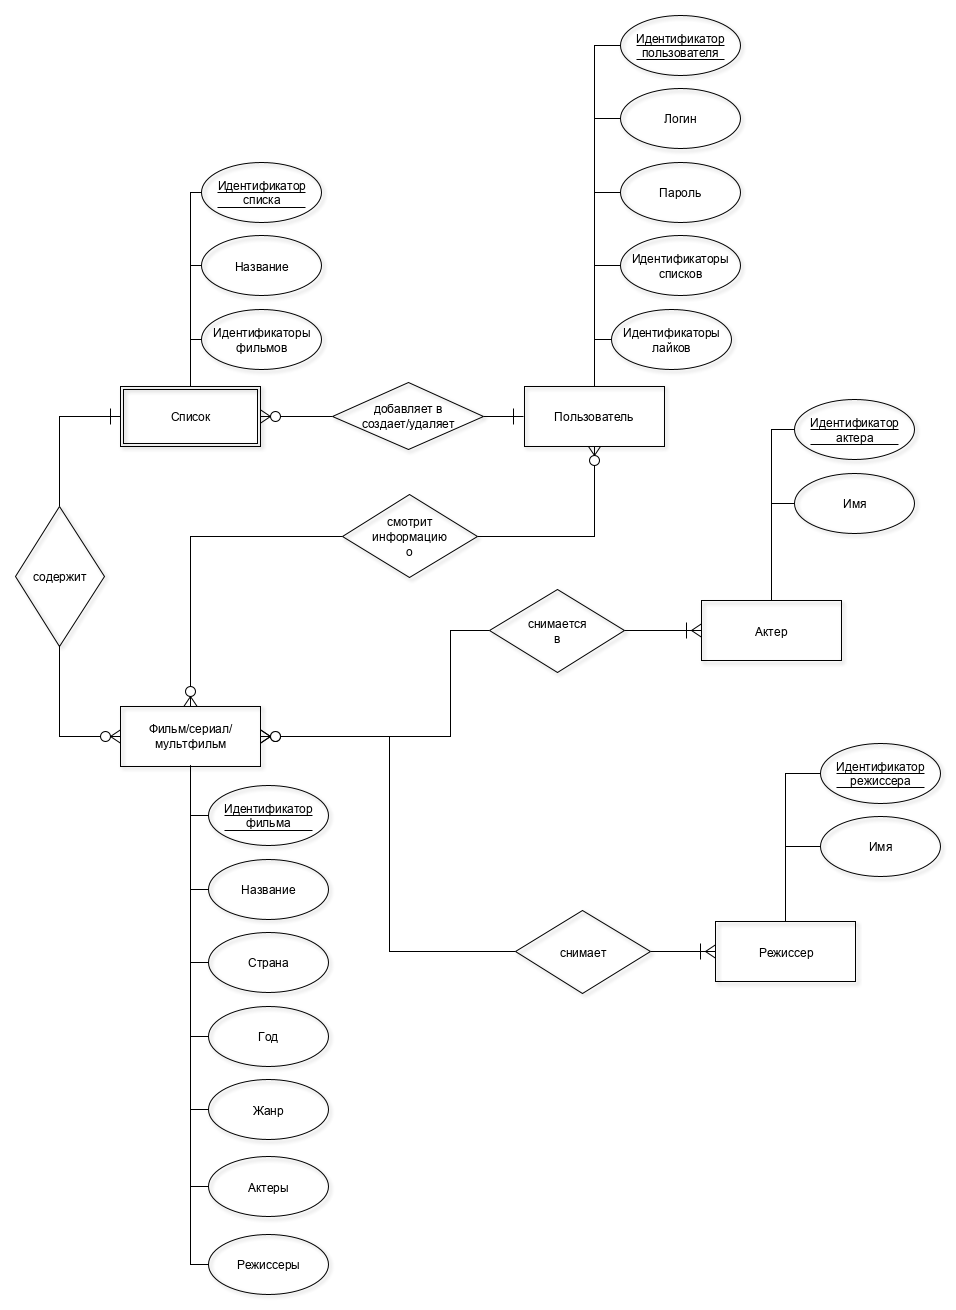
\includegraphics[scale=0.5]{img/er.png}}
		\caption{Er модель}
		\label{er-model}
	\end{figure}
	
	\subsection{Проектирование таблиц базы данных}
	
	База данных приложения <<ХочуПосмотреть!>> состоит из следующих таблиц:
	\begin{itemize}
		\item таблица пользователей сайта {\bf User};
		\item таблица актеров {\bf Actor};
		\item таблица режиссеров {\bf Director};
		\item таблица фильмов {\bf Film};
		\item таблица избранных фильмов {\bf List};
	\end{itemize}
	
	\hfill \break
	
	{\bf Таблица User}
	
	Позволяет однозначно идентифицировать пользователя сайта, реализовать авторизацию пользователя. Имеет связь <<один-ко-многим>> с таблицей List. 
	
	Таблица содержит следующие поля:
	\begin{itemize}
		\item username - символьное поле, имя пользователя;
		\item email - символьное поле, адрес электронной почты клиента;
		\item password hash - символьное поле, хэш пароля пользователя;
	\end{itemize}
	
	\hfill \break
	
	{\bf Таблица Actor}
	
	Хранит данные о актере. Связана с таблицей фильмов Film <<многие-ко-многим>>.
	
	Таблица содержит следующие поля:
	\begin{itemize}
		\item actor\_id - целочисленное поле, идентификатор актера;
		\item name - символьное поле, имя актера;
	\end{itemize}
	
	\hfill \break
	
	{\bf Таблица Director}
	
	Хранит данные о режиссере. Связана с таблицей фильмов Film <<многие-ко-многим>>.
	
	Таблица содержит следующие поля:
	\begin{itemize}
		\item actor\_id - целочисленное поле, идентификатор режиссера;
		\item name - символьное поле, имя режиссера;
	\end{itemize}
	
	\hfill \break
	
	{\bf Таблица Film}
	
	В данной таблице хранятся данные о фильмах. 
	
	Таблица содержит следующие поля:
	\begin{itemize}
		\item id – целочисленное поле, идентификатор фильма;
		\item name – символьное поле, название фильма;
		\item description – текстовое поле, описание фильма;
		\item country - символьное поле, название страны;
		\item genre - целочисленное поле, жанр фильма;
		\item actors – поле, в котором хранятся id актеров, которые снимаются в этом фильме;
		\item directors – поле, в котором хранятся id режиссеров, которые снимали этот фильм;
	\end{itemize}
	
	\hfill \break
	
	{\bf Таблица List}
	
	Таблица, содержащая фильмы, которые находятся в избранном у пользователя. С помощью связи <<один-к-одному>> связана с таблицей пользователей User.
	
	Таблица содержит следующие поля:
	\begin{itemize}
		\item id – целочисленное поле, идентификатор списка избранного;
		\item user\_id – символьное поле, username пользователя;
		\item films – поле, в котором содержатся id фильмов, которые входят в данный список избранного;
	\end{itemize}

	\begin{figure}[h!]
	\center{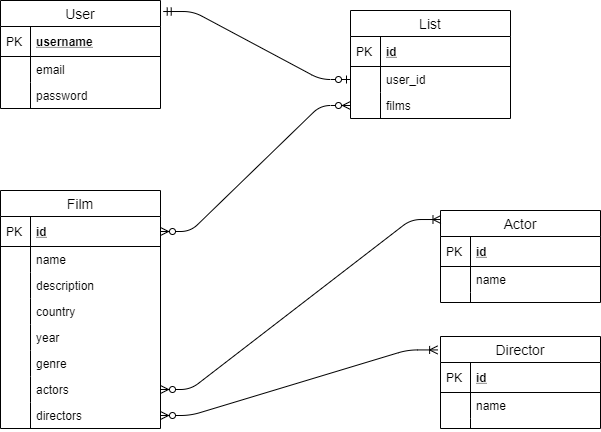
\includegraphics[scale=0.6]{img/4.png}}
	\caption{Диаграмма БД}
	\label{image0}
	\end{figure}

	\subsection{Проектирование системы изменения данных}%
	\setcounter{subsection}{2}
	
	В Django каждую таблицу представляет класс. Он отображает информацию о данных сущности. Он содержит поля и поведение данных. 
	С помощью стандартных методов осуществляются операции добавления, удаления и обновления записей.
	
	\subsection{Проектирование регистрации и аутентификации пользователя}%
	\setcounter{subsection}{3}
	
	Регистрация пользователя в приложении является добавлением в базу данных (в таблицу User) записи, содержащей необходимую информацию для аутентификации. Для этого пользователь вводит соответствующие данные  в поля регистрационной формы.
	
	Framework Django предоставляет собой набор данных базовых инструментов для реализации web-приложения. В этот функционал включена реализация аутентификации пользователя.
	
	\subsection{Вывод}
	
	Была разработана модель приложения, которое дает возможность просматривать информацию фильмов, искать по базе данных, а так же реализовывать регистрацию, аутентификацию и авторизацию пользователей.
	
	\newpage
	\section{Технологическая часть}
	
	После проектирования структуры поставленной задачи, требуется реализовать набор функций, необходимый для создания web-приложения, а также конкретизировать полный список инструментов, используемых для запуска приложения.
	
	\subsection{Выбор инструментов разработки}%
	\setcounter{subsection}{1}
	
	В ходе реализации были использованы следующие технологии и средства:
	
	\begin{itemize}
		\item язык программирования Python;
		\item СУБД SQLite;
		\item библиотека Django.
	\end{itemize}
	
	Такой набор инструментов был выбран, потому что для каждого из элементов предусмотрено взаимодействие с другими.
	Также данные инструменты полностью выполняют задачи, необходимые для реализации проекта.
	
	Использован компьютер с операционной системой Windows 10.
	
	\subsection{Реализация хранения данных}
	
	Для работы с базой данных требуется объявить классы таблиц БД.
	
	В Django существует пользовательская модель User, которая и использовалась в данном курсовом проекте. Поэтому не было необходимости в написании собственного класса пользователя.
	
	\lstset{ %
        language=C,                 % выбор языка для подсветки (здесь это С)
        basicstyle=\small\sffamily, % размер и начертание шрифта для подсветки кода
        numbers=left,               % где поставить нумерацию строк (слева\справа)
        numberstyle=\tiny,           % размер шрифта для номеров строк
        stepnumber=1,                   % размер шага между двумя номерами строк
        numbersep=-5pt,                % как далеко отстоят номера строк от         подсвечиваемого кода
        backgroundcolor=\color{white}, % цвет фона подсветки - используем         \usepackage{color}
        showspaces=false,            % показывать или нет пробелы специальными     отступами
        showstringspaces=false,      % показывать или нет пробелы в строках
        showtabs=false,             % показывать или нет табуляцию в строках
        frame=single,              % рисовать рамку вокруг кода
        tabsize=2,                 % размер табуляции по умолчанию равен 2 пробелам
        captionpos=t,              % позиция заголовка вверху [t] или внизу [b] 
        breaklines=true,           % автоматически переносить строки (да\нет)
        breakatwhitespace=false, % переносить строки только если есть пробел
        escapeinside={\%*}{*)},   % если нужно добавить комментарии в коде
	    keywordstyle=\color{blue}\ttfamily,
	    stringstyle=\color{red}\ttfamily,
	    commentstyle=\color{green}\ttfamily,
	    morecomment=[l][\color{magenta}]{\#},
	    columns=fullflexible }
    
	\begin{lstlisting}[label=some-code,caption=Класс <<Актер>>]
	class Actor(models.Model):
		name = models.CharField(max_length = 150, unique = True)
		
		def __str__(self):
			return self.name
		
		def save(self, *args, **kwargs):
			print("Actor is saved!")
			super().save(*args, **kwargs)
	\end{lstlisting}
	
	\begin{lstlisting}[label=some-code,caption=Класс <<Режиссер>>]
	class Director(models.Model):
		name = models.CharField(max_length = 150, unique = True)
		
		def __str__(self):
			return self.name
		
		def save(self, *args, **kwargs):
			print("Director is saved!")
			super().save(*args, **kwargs)
	\end{lstlisting}
	
	\newpage
	\begin{lstlisting}[label=some-code,caption=Класс <<Фильм>>]
	class Film(models.Model):	
		name = models.CharField(max_length = 100)
		description = models.TextField()
		country = models.CharField(max_length = 100)
		year = models.PositiveSmallIntegerField()
		genre = models.IntegerField(choices = GENRE)
		actors = models.ManyToManyField(Actor)
		directors = models.ManyToManyField(Director)
		
		def __str__(self):
			return self.name
		
		def save(self, *args, **kwargs):
			print("Film is saved!")
			super().save(*args, **kwargs)
		
		def getactors(self):
			return self.actors
			
		def getderecors(self):
			return self.directors
	\end{lstlisting}
	
	\begin{lstlisting}[label=some-code,caption=Класс <<Список>>]
	class List(models.Model):
		user_id = models.ForeignKey(User, on_delete=models.CASCADE)
		films = models.ManyToManyField(Film)
		
		def addtolist(self, film_id):
			self.films.add(film_id)
			self.save()
		
		def deletefromlist(self, film_id):
			self.films.remove(film_id)
			self.save()
			
		def save(self, *args, **kwargs):
			print("List is saved!")
			super().save(*args, **kwargs)
	\end{lstlisting}
	
	\subsection{Frontend-разработка}
	
	Пользовательский интерфейс при разработке web-приложения представляет из себя полноценную верстку проекта. Для этого использовалась технология Bootstrap. \\
	
	Bootstrap - это инструментарий с открытым исходным кодом для разработки web-приложений с помощью HTML, CSS и JS. Включает в себя HTML- и CSS-шаблоны оформления для типографики, веб-форм, кнопок, меток, блоков навигации и прочих компонентов веб-интерфейса, включая JavaScript-расширения. C помощью него настроен дизайн сайта.  \cite{3} \\
	
	Django предоставляет инструмент шаблонизатора, который дает возможность вносить динамические данные в html с backend. С помощью шаблонизатора есть возможность проверять данные, изменяя элементы страницы в зависимости от результата проверки.
	
	При рендеринге шаблона переменные в двойных фигурных скобках будут заменяться на вычисленные значения.
	
	Продемонстрируем действие шаблонизатора на примере шаблона вывода результатов поиска. Шаблон проверяет с помощтю шаблонизатора \{\% if object\_list \%\}, есть ли результат поиска, если есть, то с помощью шаблонизатора \{\% for film in object\_list \%\} выводит на страницу фильмы. Если же результата  нет, то пользователь увидит надпись "Ничего не найдено".
	
	\newpage
	\begin{lstlisting}[label=some-code,caption=Шаблон search\_results.html]
	
	
	<title>Films:</title>
	
	<h2>Search results:</h2>
	<div class="results">
		<ul>
		
			
			<li>
				<a href="../film{{ film.id }}">{{ film.name }}</a>
			</li>
			
		
			<h3>Nothing is found(</h3>
		
		</ul>
	</div>
	
	\end{lstlisting}
	
	Все шаблоны используют базовый шаблон \{\% extends "index.html" \%\} для избежания дублирования кода.
	
	\begin{lstlisting}[label=some-code,caption=Шаблон search\_results.html]
	
	<!DOCTYPE html>
	<html lang="ru">
	<head>
		<meta charset="UTF-8">
		<title>New in cinemaworld:</title>
		<link type="text/css" href="" rel="stylesheet" >
		<link href="https://fonts.googleapis.com/css2?family=Open+Sans" rel="stylesheet">
	</head>
	<body>
		<header>
			<div class="headerlogo">IWnannaSeeIt!</div>
			<nav>
				<div class="topnav" id="myTopNav">
				<a href="../about">ABOUT</a>
				<a href="../search">SEARCH</a>
				<a href="../app">HOME</a>
				
				<a href="">{{ user.username }}</a>
				<a href="../saved">SAVED</a>
				<a href="">LOGOUT</a>
				
				<a href="">LOGIN</a>
				<a href="">REGISTER</a>
				
				</div>
			</nav>
		</header>
		<div class="main">
			
			
		</div>
	</body>
	</html>
	\end{lstlisting}
	\newpage
	
	\subsection{Интерфейс приложения}
	
	Незарегистрированные пользователи могут просматривать информацию о фильмах и совершать поиск по различным параметрам. У зарегистрированного пользователя, помимо перечисленных функций есть также возможность добавлять понравившиеся фильмы в избранное.
	
	На рисунке \ref{reg} прлдемонстрирована форма регистрации пользователя, а на рисунке \ref{login} - форма авторизации.
	
	\begin{figure}[h!]
		\center{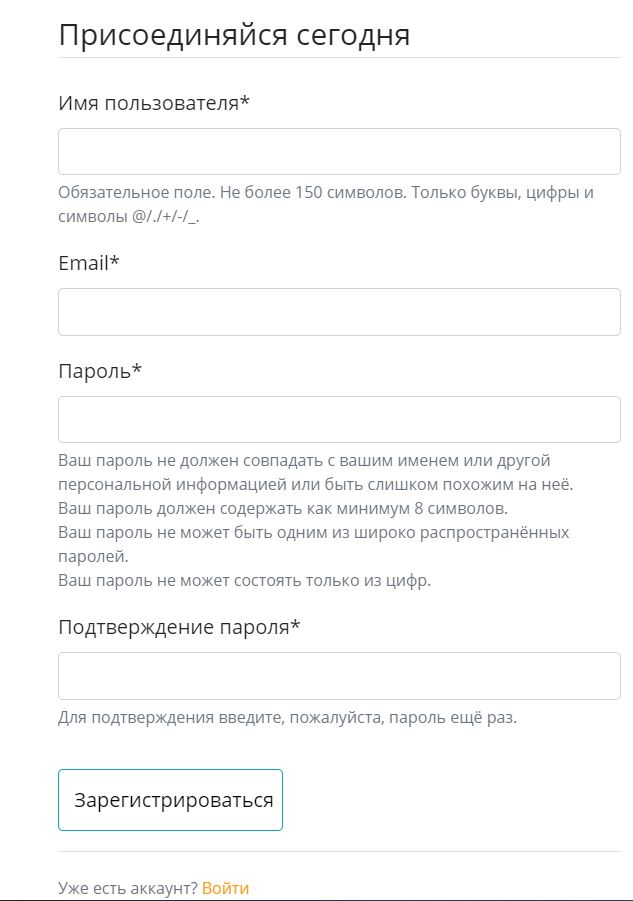
\includegraphics[scale=0.8]{img/6.JPG}}
		\caption{Страница регистрации}
		\label{reg}
	\end{figure}
	
	\newpage
	\begin{figure}[h!]
		\center{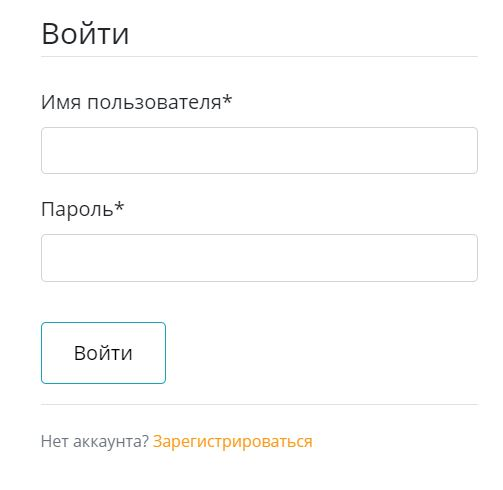
\includegraphics[scale=0.7]{img/5.JPG}}
		\caption{Страница авторизации}
		\label{login}
	\end{figure}

	На рисунках \ref{home1} и \ref{home2} продемонстрирована главная страница приложения, где можно увидеть новинки кино и ссылки на эти фильмы для просмотра информации о них. Единственное отличие между данными рисунками, это то, что на \ref{home1} главная страница незарегистрированного пользователя, можно заметить ссылки на авторизацию и регистрацию в правом верхне углу. На рисунке \ref{home2} пользователь авторизирован, поэтому перечисленных ранее ссылок нет, вместо этого можно увидеть имя пользователя, ссылку на Избранное и кпопку выхода из учетной записи.

	\begin{figure}[h!]
		{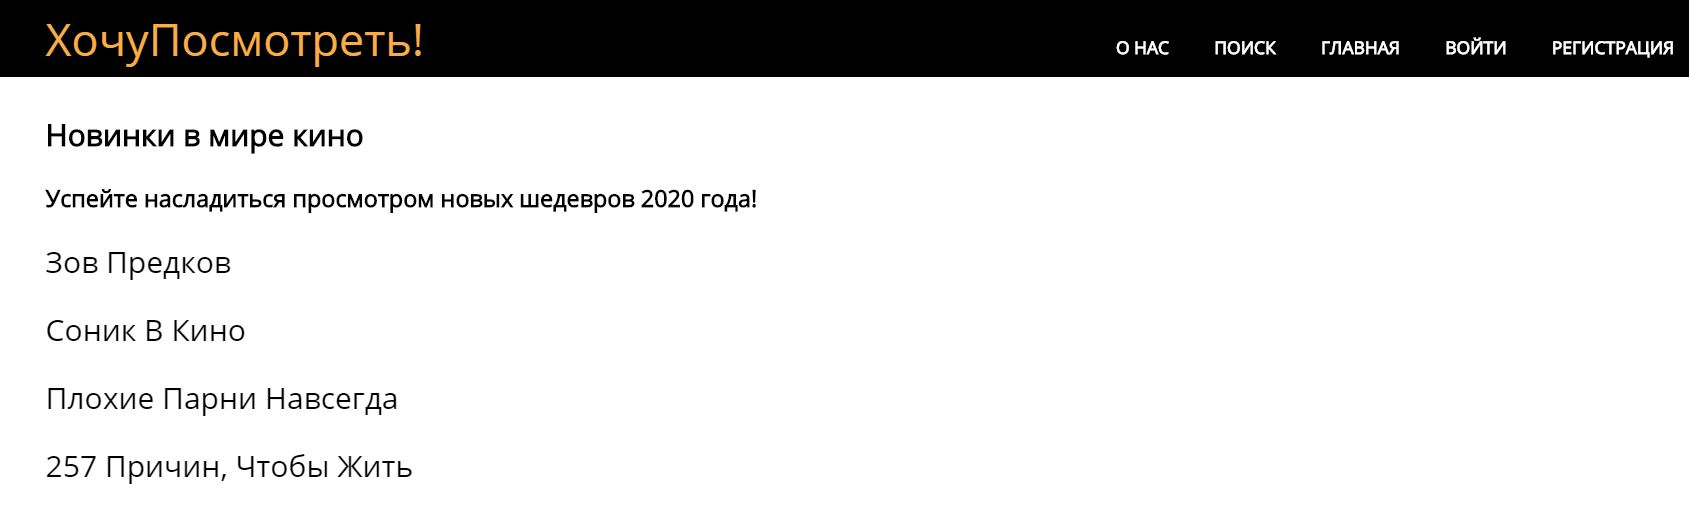
\includegraphics[scale=0.5]{img/7.JPG}}
		\caption{Главная страница незарегистрированного пользователя}
		\label{home1}
	\end{figure}
	
	\newpage
	\begin{figure}[h!]
		{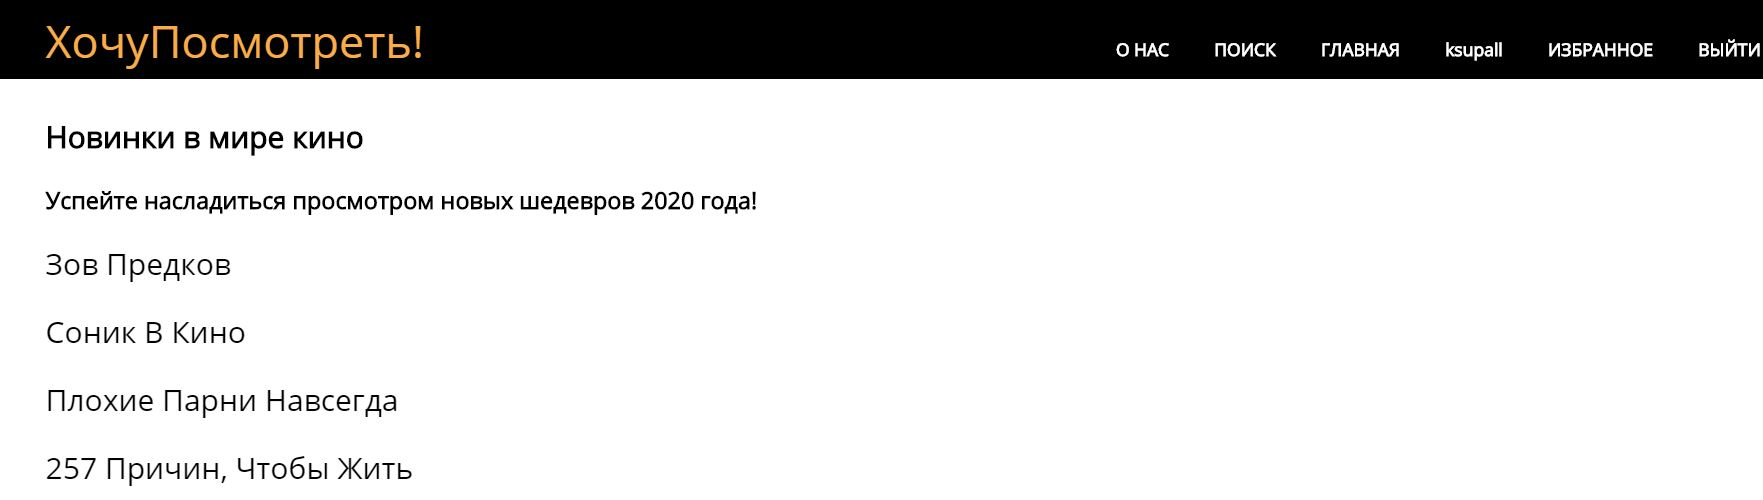
\includegraphics[scale=0.5]{img/8.JPG}}
		\caption{Главная страница зарегистрированного пользователя}
		\label{home2}
	\end{figure}

	На рисунке \ref{saved1} приведен пример, когда раздел "Избранное" пуст. Шаблонизатор, о котором говорилось выше, выводит сообщение "Нет фильмов!".
	
	\begin{figure}[h!]
		{
\includegraphics[scale=0.6]{img/9.JPG}}
		\caption{Раздел "Избранное" пуст}
		\label{saved1}
	\end{figure}

	На рисунке \ref{search} продемонстрирована форма поиска. Данная функция доступна как зарегистрированным пользователям, так и незарегистрированным. Форма состоит из нескольких текстовых полей, а так же радиокнопок для выбора жанра. Поиск можно выполнить как по одному параметру, например, по жанру, так и по нескольким параметрам сразу. Если же никакие параметры введены не будут, то поиск выдаст все фильмы, которые находятся в базе данных. Для очистки полей рядом с кнопкой "Искать" расположена кнопка "Очистить".
	\newpage

	\begin{figure}[h!]
		\center{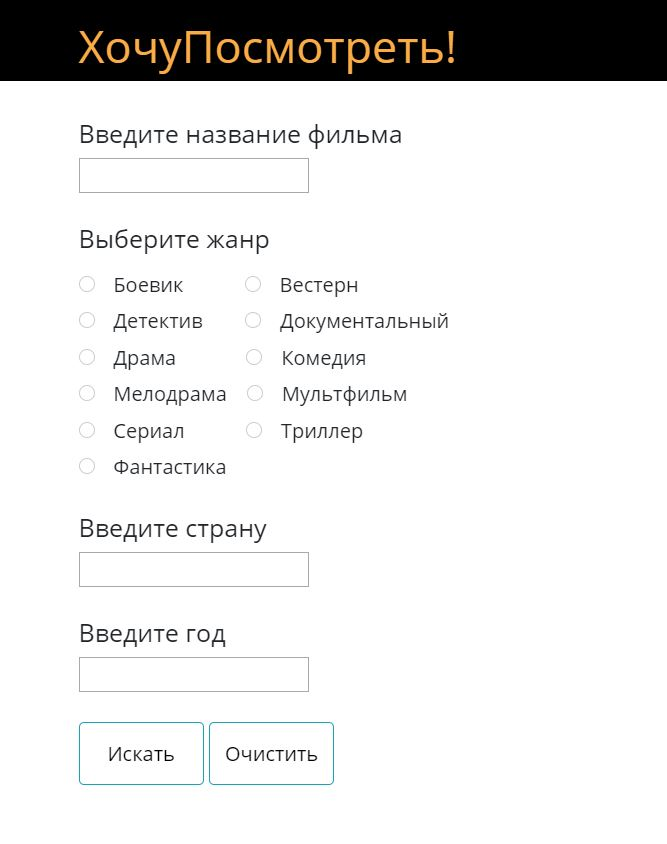
\includegraphics[scale=0.7]{img/10.JPG}}
		\caption{Форма поиска}
		\label{search}
	\end{figure}

	На рисунке \ref{res} представлен результат поиска. В качестве результата можно увидеть список фильмов, которые были подобраны по некоторым параметрам. Список состоит из ссылок, поэтому после поиска можно посмотреть более подробную информацию о каждом фильме.
	
	\newpage
	\begin{figure}[h!]
		\center{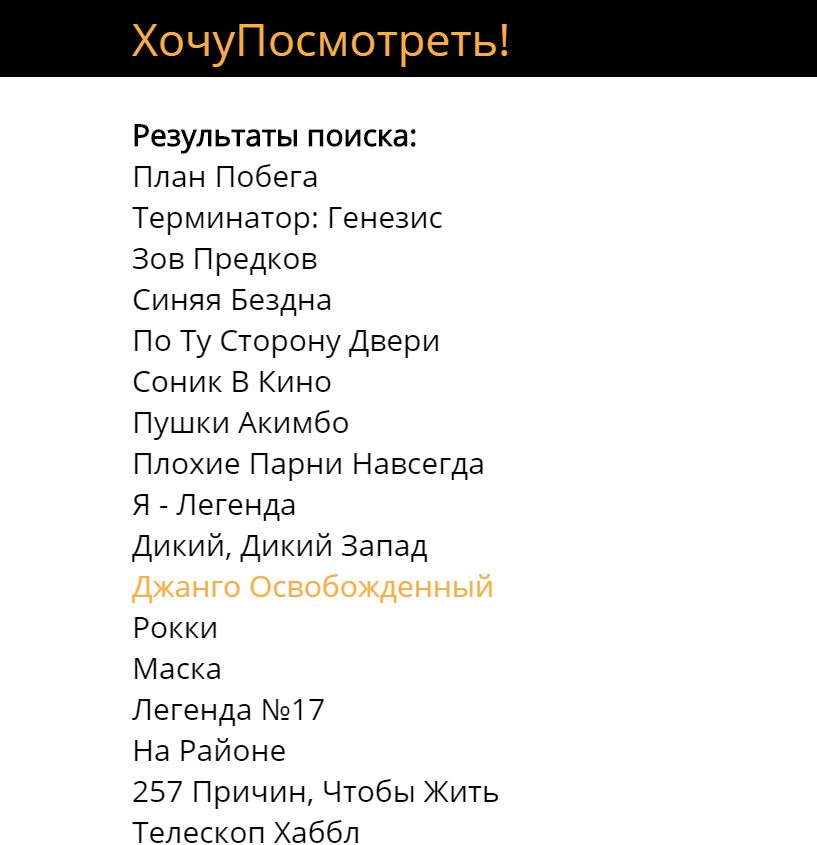
\includegraphics[scale=0.7]{img/11.JPG}}
		\caption{Результат поиска}
		\label{res}
	\end{figure}
	
	На рисунке \ref{film} представлена страница фильма. Здесь находится вся информация о фильме: название, описание, страна, год премьеры, жанр, режиссер и актеры, которые в нем снимались. Ниже данной информации можно увидеть кнопку "Добавить" , она выполняет добавление данного фильма в избранное. Если этот фильм уже есть в избранном, то вместо кпопки "Добавить" будет кпопка "Удалить". Страница с фильмом, который уже находится в Избранном, продемонстрирована на рисунке \ref{film2}. Однако данная функция добавления в Избранное доступна только зарегистрированным пользователям, поэтому у незарегистрированных пользователей кнопок не будет вовсе.		
	
	\begin{figure}[h!]
		\center{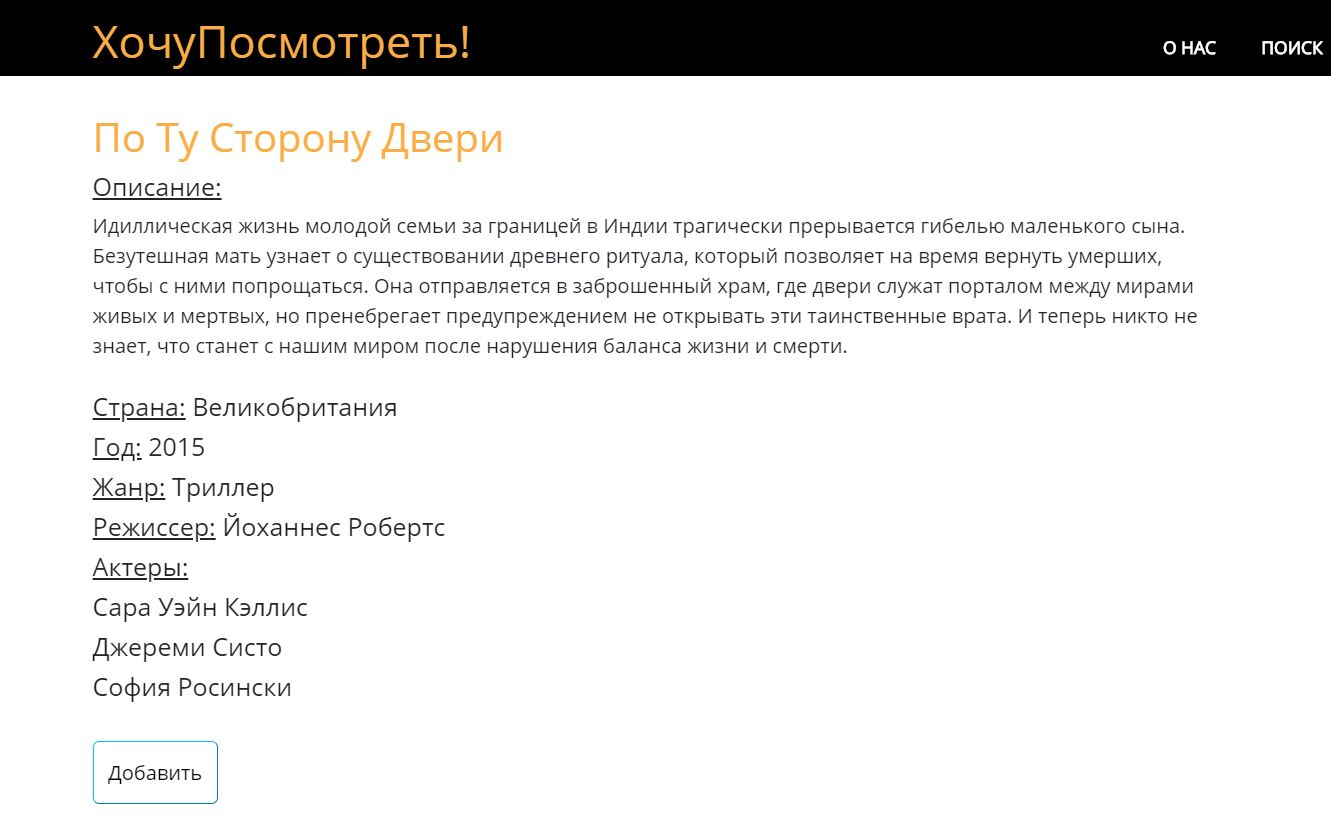
\includegraphics[scale=0.63]{img/12.JPG}}
		\caption{Страница фильма с кнопкой "Добавить"}
		\label{film}
	\end{figure}

	\begin{figure}[h!]
		\center{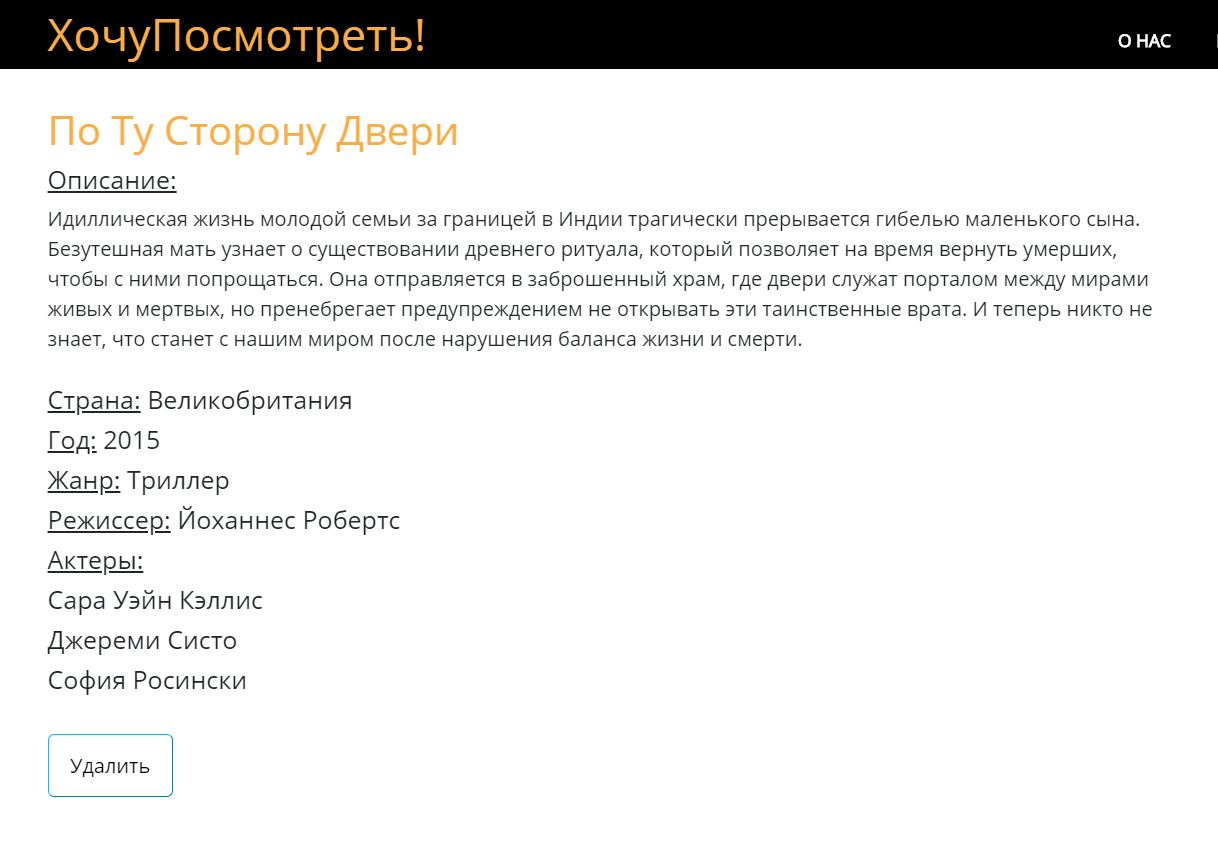
\includegraphics[scale=0.63]{img/14.JPG}}
		\caption{Страница фильма с кнопкой "Удалить"}
		\label{film2}
	\end{figure}
	\newpage
	
	\subsection{Вывод}
	В данной части был выбран набор инструментов был для реализации поставленной задачи. Также были приведены листинги классов для формирования таблиц базы данных. В данной части был рассмотрен интерфейс приложения и основные его функции.
	
	\newpage
		
	\section*{Заключение}
	\addcontentsline{toc}{section}{Заключение}
	
	В результате проделанной работы:
	\begin{itemize}
		\item были продуманы функции, которые должно было решать приложение;
		\item проведен анализ инструментов, необходимых для проектирования и реализации задачи, в результате которого был выбраны такие инструменты, как SQLite, Flask;
		\item разработана структура базы данных, состоящая их нескольких сущностей;
		\item с помощью выбранных инструментов был реализован web-интерфейс, обладающий возможностью регистрировать пользователей, изменять состояние и местоположение книг, добавлять и удалять книги, а также осуществлять поиск по ключевым словам.
	\end{itemize}	
	\newpage
	
	\addcontentsline{toc}{section}{Список используемой литературы}
	\begin{thebibliography}{3}
		
		\bibitem{0} Интернет технологии [Электронный ресурс]
		URL: \underline{https://www.internet-technologies.ru/articles/modeli-...}
		\underline{upravleniya-bazami-dannyh.html} (Дата обращеня: 28.05.2020)
		\hfill \break
		
		\bibitem{1} 
		Документация Sqlite [Электронный ресурс]
		URL: \underline{https://www.sqlite.org} (Дата обращеня: 28.05.2020)
		\hfill \break
		
		\bibitem{mvc} MVC [Электронный ресурс]
		URL: \underline{https://tproger.ru/articles/mvc/} (Дата обращеня: 28.05.2020)
		\hfill \break
		
		\bibitem{3} Bootstrap [Электронный ресурс] URL: \underline{https://bootstrap-4.ru}  (Дата обращеня: 19.09.2019)
		
		\bibitem{2} Документация Django [Электронный ресурс]
		URL: \underline{https://docs.djangoproject.com/en/3.0/} (Дата обращеня: 28.05.2020)
		\hfill \break
		
	\end{thebibliography}

    
\end{document}